\documentclass[aspectratio=169,10pt]{beamer}

\usepackage[utf8]{inputenc}
\usepackage[T1]{fontenc}
\usepackage[english]{babel}
\usepackage{lmodern}
\usepackage{amsmath,amssymb}
\usepackage{booktabs}
\usepackage{graphicx}
\usepackage{array}
\usepackage{xcolor}

% Tema y colores institucionales (FP-UNA)
\usetheme{Madrid}
\usecolortheme{whale}
\definecolor{fpunablue}{RGB}{15, 52, 96}
\definecolor{fpunaaccent}{RGB}{22, 105, 122}
\definecolor{fpunagreen}{RGB}{27, 115, 64}
\setbeamercolor{structure}{fg=fpunablue}
\setbeamercolor{palette primary}{bg=fpunablue,fg=white}
\setbeamercolor{palette secondary}{bg=fpunaaccent,fg=white}
\setbeamercolor{palette tertiary}{bg=fpunablue,fg=white}
\setbeamercolor{titlelike}{parent=palette primary}
\setbeamercolor{block title}{bg=fpunablue,fg=white}
\setbeamercolor{block body}{bg=fpunablue!6,fg=black}
\setbeamercolor{block title alerted}{bg=red!70!black,fg=white}
\setbeamercolor{block body alerted}{bg=red!6,fg=black}
\setbeamercolor{block title example}{bg=fpunagreen,fg=white}
\setbeamercolor{block body example}{bg=fpunagreen!6,fg=black}

\setbeamertemplate{navigation symbols}{}
\setbeamertemplate{caption}[numbered]
\renewcommand{\tablename}{Tabla}
\renewcommand{\figurename}{Figura}

\title[Defensa de Tesis — FSC-Tex]{Concatenación sistemática y fusión adaptativa costo-consciente de descriptores visuales para clasificación de texturas}
\subtitle{De la selección anidada de bloques a la adquisición secuencial guiada por incertidumbre}
\author[C. Ayala \& J. Delgado]{\textbf{Carlos Ayala} \and \textbf{Joaquín Delgado} \\[0.4em] {\small Tutor: Prof. José Vázquez}}
\institute[FP-UNA]{Universidad Nacional de Asunción \\ Facultad Politécnica}
\date[Octubre 2026]{Octubre 2026}

\begin{document}

% =========================================================================
% DIAPOSITIVA 1: PORTADA
% =========================================================================
\begin{frame}
\titlepage
\end{frame}

% =========================================================================
% DIAPOSITIVA 2: AGENDA
% =========================================================================
\begin{frame}{Estructura de la Presentación}
\begin{columns}[T]
\begin{column}{0.48\textwidth}
\begin{block}{Parte I: Fundamentos y Concatenación Estática}
\begin{enumerate}
\item \textbf{Motivación y Problema:} Diversidad textural frente al costo de extracción.
\item \textbf{Preguntas y Aportes:} Del análisis estático a la inferencia condicional.
\item \textbf{Biblioteca de 22 Descriptores:} 6 clásicos + 16 profundos/fundacionales (20.652 dims).
\item \textbf{Protocolo Anidado y Fase 1:} Evaluación en 6 conjuntos con Linear SVM y ResMLP.
\end{enumerate}
\end{block}
\end{column}
\begin{column}{0.48\textwidth}
\begin{block}{Parte II: Cascada Adaptativa y Comparación con el Estado del Arte}
\begin{enumerate}\setcounter{enumi}{4}
\item \textbf{Arquitectura FSC-Tex:} Regla de decisión por margen $m(x)$ y umbral prospectivo $\tau$.
\item \textbf{Evaluación en 27 Condiciones:} Desempeño macro-F1 por dataset y pruebas de Demšar.
\item \textbf{Validación Física en GPU (RTX 4060):} 612 pares estratificados + 94/94 condiciones online.
\item \textbf{Comparación contra Literatura Reciente (2022--2026):} 4 arquitecturas de concatenación en los 6 datasets.
\item \textbf{Discusión, Límites y Conclusiones.}
\end{enumerate}
\end{block}
\end{column}
\end{columns}
\end{frame}

% =========================================================================
% DIAPOSITIVA 3: MOTIVACIÓN Y PROBLEMA
% =========================================================================
\begin{frame}{1. Motivación y Problema de Investigación}
\begin{columns}[T]
\begin{column}{0.54\textwidth}
\begin{block}{Naturaleza heterogénea de las texturas visuales}
\begin{itemize}
\item Ningún descriptor aislado captura simultáneamente microestructuras locales, periodicidad espectral y semántica global de materiales.
\item Combinar operadores clásicos (LBP, Gabor, GLCM, HOG, N-gramas) con CNNs, ViTs y modelos fundacionales (DINOv2, SigLIP, BEiT-v2) eleva la capacidad discriminativa.
\end{itemize}
\end{block}
\begin{alertblock}{El cuello de botella operativo de la concatenación estática}
\begin{itemize}
\item \textbf{Saturación dimensional:} las ganancias de exactitud muestran rendimientos decrecientes tras pocos bloques de alto orden.
\item \textbf{Costo fijo invariable:} extraer 22 modelos (20.652 dims) para el \textbf{100\% de las imágenes} exige cientos de milisegundos por consulta, aun cuando la gran mayoría de las muestras son visualmente no ambiguas.
\end{itemize}
\end{alertblock}
\end{column}
\begin{column}{0.43\textwidth}
\centering
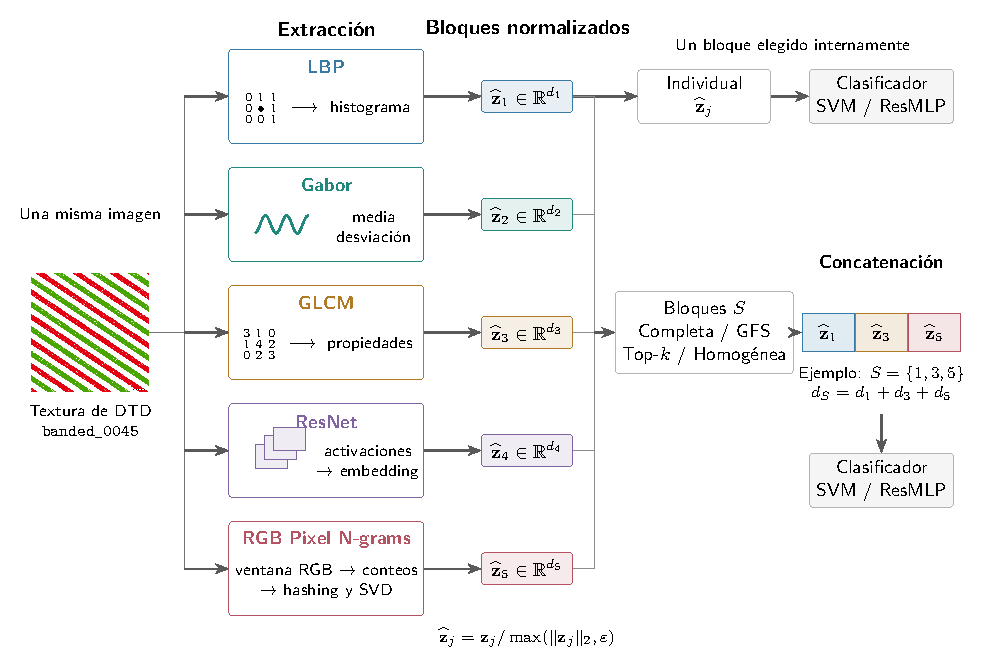
\includegraphics[width=\textwidth]{articulo/borrador_profesor/figures/concatenacion_v02.pdf}
\vspace{0.2em}
{\scriptsize Extracción heterogénea y normalización $L_2$ por bloque antes de la unión conjunta.}
\end{column}
\end{columns}
\end{frame}

% =========================================================================
% DIAPOSITIVA 4: PREGUNTAS Y APORTES
% =========================================================================
\begin{frame}{2. Preguntas de Estudio y Aportes del Trabajo}
\begin{block}{Preguntas de Investigación}
\begin{enumerate}
\item \textbf{Fase 1 (Estática):} \emph{¿En qué medida y a qué costo dimensional la concatenación estática de bloques supera la selección del mejor descriptor individual, y cuál es el impacto de la política de composición del subconjunto?}
\item \textbf{Fase 2 (Dinámica):} \emph{¿Es posible aproximar estrechamente la calidad predictiva de la concatenación densa reduciendo sustancialmente el tiempo de inferencia mediante una regla adaptativa de adquisición secuencial guiada por incertidumbre?}
\end{enumerate}
\end{block}

\begin{exampleblock}{Aportes Verificables de la Tesis}
\begin{itemize}
\item \textbf{Aporte 1:} Evaluación anidada sin fuga de 5 estrategias estáticas sobre \textbf{22 descriptores (20.652 dims)} y \textbf{6 datasets} con dos clasificadores (Linear SVM y ResMLP), más reglas de selección de ensamble por diversidad y ganancia marginal.
\item \textbf{Aporte 2:} Formulación y evaluación de la \textbf{Cascada Adaptativa Costo-Consciente} (2 etapas guiadas por margen OOF) en las 27 condiciones canónicas y en el panel online completo de \textbf{94/94 condiciones (362.640 llamadas físicas)}.
\item \textbf{Aporte 3:} \textbf{Benchmark físico pareado en GPU (NVIDIA RTX 4060)} sobre los \textbf{6 datasets} (\textbf{612 mediciones pareadas}): \textbf{69,0\% menos latencia} (\textbf{3,23$\times$}) y \textbf{100\% de paridad con caché}.
\item \textbf{Aporte 4:} \textbf{Adaptación fiel y comparación directa en los 6 datasets contra 4 métodos recientes de concatenación} (\textbf{Neshov 2025}, \textbf{DeepLumina 2022}, \textbf{HyTexNet 2026} y \textbf{6LBP+dCellNN 2024}, sumando \textbf{141.584 inferencias online adicionales}).
\end{itemize}
\end{exampleblock}
\end{frame}

% =========================================================================
% DIAPOSITIVA 5: BIBLIOTECA DE 22 DESCRIPTORES
% =========================================================================
\begin{frame}{3. Espacio de Representación: Biblioteca de 22 Descriptores}
\begin{columns}[T]
\begin{column}{0.44\textwidth}
\begin{table}
\centering
\scriptsize
\caption{6 Descriptores Clásicos y de Color (2.220 dims)}
\begin{tabular}{@{}llr@{}}
\toprule
Descriptor & Parametrización & Dim. \\
\midrule
LBP & Multiescala $(8,1),(16,2),(24,3)$ riu2 & 54 \\
LBP-rot (\texttt{drlbp}) & $P=8, R=1$, 8 rotaciones $[0,10]$ & 80 \\
Gabor & 4 frecuencias, 6 orientaciones & 48 \\
GLCM & 256 niveles, dist. 1--3, 4 ángulos & 18 \\
HOG & 9 orient., celda $16^2$, bloque $2^2$ & 1.764 \\
RGB N-gramas+SVD & Ventana $2\times 1$, 8.192 bins, SVD & 256 \\
\bottomrule
\end{tabular}
\end{table}
\vspace{-0.3em}
\begin{block}{\scriptsize Normalización Conjunta por Bloque}
\centering
$\displaystyle \mathbf{z}_{i,S}=\mathop{\Vert}_{j\in S}\frac{\mathbf{z}_{ij}}{\max(\lVert\mathbf{z}_{ij}\rVert_2,10^{-12})}, \quad d_{\text{total}} = 20.652$
\end{block}
\end{column}
\begin{column}{0.53\textwidth}
\begin{table}
\centering
\scriptsize
\caption{16 Extractores Profundos y Fundacionales (18.432 dims)}
\begin{tabular}{@{}lllr@{}}
\toprule
Familia & Modelos Incluidos & Salida & Dim. \\
\midrule
CNN (6) & VGG16 (4096), ResNet-50 (2048), & Preclas. & 11.264 \\
        & ResNet-101 (2048), DenseNet-121 (1024), & & \\
        & EfficientNet-B0 (1280), ConvNeXt V2-T (768) & & \\
\midrule
ViT (5) & ViT-B/16 (768), DeiT-S (384), Swin-T (768), & Pooler/ & 3.456 \\
        & EVA-02-B (768), BEiT-v2-B (768) & CLS & \\
\midrule
Autosup./ & DINOv2-S (384), DINOv2-B (768), & Pooler/ & 3.712 \\
Multim. (5) & DINOv2-L (1024), MAE-B (768), & Preclas. & \\
        & SigLIP-B (768) & & \\
\bottomrule
\end{tabular}
\end{table}
\end{column}
\end{columns}
\end{frame}

% =========================================================================
% DIAPOSITIVA 6: ESTRATEGIAS ESTÁTICAS Y PROTOCOLO ANIDADO
% =========================================================================
\begin{frame}{4. Estrategias Estáticas Comparadas y Selección Anidada}
\begin{columns}[T]
\begin{column}{0.52\textwidth}
\begin{block}{Cinco Controles Estáticos Evaluados}
\begin{enumerate}
\item \textbf{Individual:} Mejor bloque único en validación interna.
\item \textbf{Completa-22:} Unión de los 22 bloques (20.652 dims).
\item \textbf{Top-$k$:} Concatenación de los $k$ mejores individuales internos ($k$ igualado al tamaño de GFS).
\item \textbf{GFS (\emph{Greedy Forward Selection}):} Adición voraz paso a paso hasta $k \le 8$ (parada tras dos mejoras $< 0{,}001$).
\item \textbf{Homogénea:} Mejor GFS restringido a una sola familia.
\end{enumerate}
\end{block}
\begin{exampleblock}{\scriptsize Aislamiento Estricto (Cero Fuga de Datos)}
Toda selección de bloques, ajuste de SVD y normalización se ejecuta exclusivamente en los 4 pliegues internos de $T_{\text{train}}$. El test externo se evalúa una única vez.
\end{exampleblock}
\end{column}
\begin{column}{0.45\textwidth}
\centering
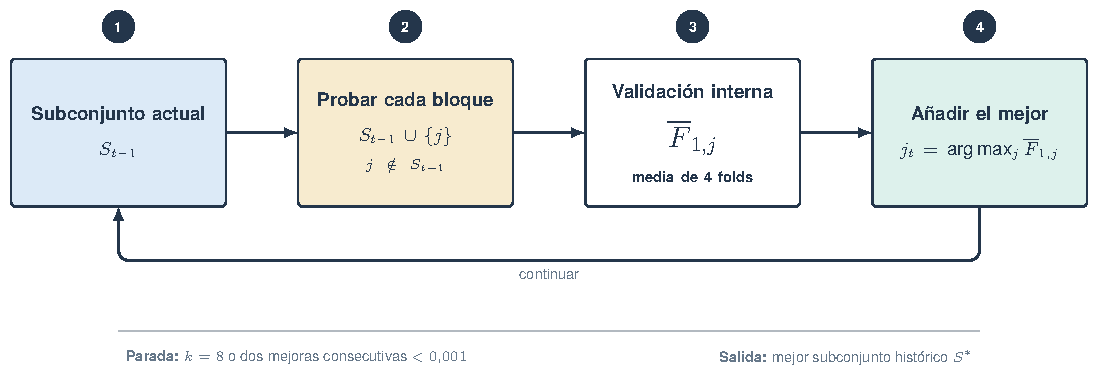
\includegraphics[width=\textwidth]{articulo/borrador_profesor/figures/gfs_pasos.pdf}
\vspace{0.2em}
{\scriptsize Esquema de selección anidada de bloques mediante GFS dentro de $T_{\text{train}}$.}
\end{column}
\end{columns}
\end{frame}

% =========================================================================
% DIAPOSITIVA 7: DATASETS Y DISEÑO EXPERIMENTAL
% =========================================================================
\begin{frame}{5. Conjuntos de Datos y Cobertura Experimental}
\begin{table}
\centering
\footnotesize
\caption{Seis conjuntos de datos de referencia evaluados en la tesis}
\begin{tabular}{@{}llrrll@{}}
\toprule
Conjunto de Datos & Dominio Textural & Imágenes & Clases & Protocolo Fase 1 (Estática) & Protocolo Fase 2 (Cascada) \\
\midrule
\textbf{DTD} & Texturas en la naturaleza (\emph{in-the-wild}) & 5.640 & 47 & 10 splits oficiales & 10 splits oficiales \\
\textbf{FMD} & Categorías de materiales (Flickr) & 1.000 & 10 & 5 folds $\times$ 3 semillas (15) & 5 folds canónicos (s42) \\
\textbf{CUReT} & Materiales bajo pose/iluminación variable & 5.612 & 61 & 2 direcciones (\texttt{a\_to\_b}, \texttt{b\_to\_a}) & 2 direcciones \\
\textbf{Outex13} & Texturas controladas en color (TC-00013) & 1.360 & 68 & 1 split oficial (680/680) & 1 split oficial \\
\textbf{SoilOriginal} & Texturas de suelos agrícolas deduplicados & 1.140 & 7 & 5 folds $\times$ 3 semillas (15) & 5 folds canónicos (s42) \\
\textbf{KTH-TIPS-2b} & Materiales con 4 muestras físicas (\emph{a--d}) & 4.752 & 11 & 4 splits invertidos (\texttt{innergrp}) & 4 splits invertidos \\
\bottomrule
\end{tabular}
\end{table}

\begin{itemize}
\item \textbf{Clasificadores Evaluados:}
  \begin{itemize}
  \item \textbf{Linear SVM (\texttt{LinearSVC}):} $C=1$, pesos balanceados, regularización $L_2$ (Fase 1 y Fase 2).
  \item \textbf{ResMLP:} Red residual multicapa (proyección a 256d, 3 bloques residuales, LayerNorm, GELU, AdamW) para contrastar sesgo inductivo no lineal en Fase 1.
  \end{itemize}
\end{itemize}
\end{frame}

% =========================================================================
% DIAPOSITIVA 8: RESULTADOS FASE 1
% =========================================================================
\begin{frame}{6. Resultados Fase 1: Concatenación Estática por Dataset}
\begin{columns}[T]
\begin{column}{0.56\textwidth}
\begin{table}
\centering
\scriptsize
\caption{Macro-F1 medio por conjunto de datos (22 descriptores)}
\begin{tabular}{@{}llccccc@{}}
\toprule
Modelo & Dataset & Indiv. & Completa & Top-$k$ & GFS & Homog. \\
\midrule
\textbf{SVM} & DTD & 0,8426 & 0,8639 & 0,8700 & \textbf{0,8703} & 0,8604 \\
 & FMD & 0,9726 & 0,9647 & \textbf{0,9820} & 0,9766 & 0,9789 \\
 & CUReT & 0,9948 & \textbf{0,9989} & \textbf{0,9989} & 0,9988 & \textbf{0,9989} \\
 & Outex13 & 0,9066 & \textbf{0,9656} & 0,9426 & 0,9589 & 0,9307 \\
 & SoilOriginal & 0,8578 & \textbf{0,8816} & 0,8776 & 0,8671 & 0,8670 \\
 & KTH-TIPS-2b & 0,9396 & \textbf{0,9601} & 0,9445* & 0,9355* & 0,9271 \\
\midrule
\textbf{ResMLP} & DTD & 0,8379 & 0,8622 & \textbf{0,8643} & 0,8640 & 0,8538 \\
 & FMD & 0,9689 & 0,9714 & \textbf{0,9766} & 0,9763 & 0,9726 \\
 & CUReT & 0,9951 & \textbf{0,9991} & 0,9990 & 0,9990 & 0,9989 \\
 & Outex13 & 0,9179 & 0,9661 & 0,9580 & \textbf{0,9715} & 0,9337 \\
 & SoilOriginal & 0,8532 & 0,8606 & 0,8678 & \textbf{0,8691} & 0,8558 \\
 & KTH-TIPS-2b & 0,9061 & \textbf{0,9487} & 0,9322 & 0,9201 & 0,9127 \\
\bottomrule
\end{tabular}
\end{table}
{\tiny *En KTH con SVM: Top-$k$ corregido (\texttt{innergrp-sample}, 4 folds) = 0,9445 (archivo original = 0,9350).}
\end{column}
\begin{column}{0.42\textwidth}
\begin{block}{\scriptsize Pruebas de Demšar por Clasificador ($N=6$)}
\scriptsize
\begin{itemize}
\item \textbf{Friedman / Iman--Davenport:}
  \begin{itemize}
  \item \scriptsize \textbf{SVM:} $p = 0{,}0289$ / $p = 0{,}0139$. Mejor rango: Completa y Top-$k$ ($2{,}000$).
  \item \scriptsize \textbf{ResMLP:} $p = 0{,}0110$ / $p = 0{,}0025$. Mejor rango: \textbf{GFS ($1{,}667$)}.
  \end{itemize}
\item \textbf{Ajuste de Holm (10 pares):}
  \begin{itemize}
  \item \scriptsize \textbf{ResMLP:} GFS supera significativamente a Individual ($p_{\text{Holm}} = \mathbf{0{,}0191}$).
  \item \scriptsize \textbf{SVM:} Top-$k$ y Completa vs. Individual obtienen $p_{\text{Holm}} = 0{,}0617$.
  \end{itemize}
\item \textbf{Contracción dimensional:} GFS reduce entre \textbf{67,1\% y 95,3\%} las dimensiones frente a las 20.652 de Completa, pero aún exige ejecutar varios modelos para cada imagen.
\end{itemize}
\end{block}
\end{column}
\end{columns}
\end{frame}

% =========================================================================
% DIAPOSITIVA 9: PROPUESTA CASCADA ADAPTATIVA FSC-TEX
% =========================================================================
\begin{frame}{7. Fase 2: Cascada Adaptativa Costo-Consciente (FSC-Tex)}
\begin{block}{Idea Central: Adquisición Condicional Guiada por Incertidumbre}
En lugar de extraer todos los descriptores del subconjunto para todas las imágenes, el sistema evalúa inicialmente un \textbf{único extractor económico} $\phi_{\text{cheap}}$ y decide en tiempo de ejecución si la predicción es confiable o si requiere escalar al conjunto denso Top-$k$.
\end{block}

\begin{columns}[T]
\begin{column}{0.48\textwidth}
\begin{exampleblock}{Etapa 1: Inferencia Económica y Salida Temprana}
\begin{itemize}
\item Se extrae el descriptor inicial $\phi_{\text{cheap}} \in \{\text{SigLIP-B}, \text{ResNet-50}, \text{BEiT-v2-B}, \text{ConvNeXt-V2-T}\}$.
\item El clasificador lineal produce el vector de puntuaciones de clase $\mathbf{s}(x) = [s_1, \dots, s_C]$.
\item Si el margen $m(x) > \tau$, se emite $\hat{y}_{\text{cheap}}(x)$ de inmediato (\textbf{74,0\% de los casos en GPU}).
\end{itemize}
\end{exampleblock}
\end{column}
\begin{column}{0.48\textwidth}
\begin{alertblock}{Etapa 2: Escalamiento Condicional Denso}
\begin{itemize}
\item Solo cuando $m(x) \le \tau$ (muestra ambigua o con incertidumbre alta, \textbf{26,0\% de los casos}), se activan los bloques restantes de $\mathcal{B}_{\text{Top-}k}$.
\item Se reutiliza el bloque inicial si pertenece a Top-$k$, se concatenan los vectores normalizados y se predice con el modelo conjunto $\hat{y}_{\text{Top-}k}(x)$.
\end{itemize}
\end{alertblock}
\end{column}
\end{columns}
\end{frame}

% =========================================================================
% DIAPOSITIVA 10: FORMULACIÓN MATEMÁTICA DE INCERTIDUMBRE Y UMBRAL
% =========================================================================
\begin{frame}{8. Cálculo del Margen de Incertidumbre y Calibración OOF}
\begin{columns}[T]
\begin{column}{0.48\textwidth}
\begin{block}{1. Margen de Confianza Muestra por Muestra}
Sean $s_{(1)}$ y $s_{(2)}$ la mayor y la segunda mayor puntuación de decisión en la Etapa 1:
\[
m(x) = s_{(1)} - s_{(2)}
\]
\begin{itemize}
\item \textbf{$m(x)$ alto:} Separación clara entre la clase líder y su competidora $\rightarrow$ \textbf{baja incertidumbre}.
\item \textbf{$m(x) \approx 0$:} Empate técnico entre dos texturas $\rightarrow$ \textbf{alta incertidumbre}.
\end{itemize}
\[
\hat{y}(x) =
\begin{cases}
\hat{y}_{\text{cheap}}(x), & \text{si } m(x) > \tau \text{ (Salida Etapa 1)} \\
\hat{y}_{\text{Top-}k}(x), & \text{si } m(x) \le \tau \text{ (Escala a Etapa 2)}
\end{cases}
\]
\end{block}
\end{column}
\begin{column}{0.48\textwidth}
\begin{block}{2. Calibración Prospectiva de $\tau$ (Cero Fuga)}
\begin{enumerate}
\item En $T_{\text{train}}$, se obtienen predicciones y márgenes fuera de pliegue (\emph{Out-of-Fold}, 4-fold StratifiedGroupKFold).
\item Para cada presupuesto candidato $B \in \{0{,}25; 0{,}50; 0{,}75\}$, el umbral se fija como el cuantil empírico:
\[
\tau_B = \text{Cuantil}_B\big(\{m_{\text{OOF}}(x_i)\}_{i \in T_{\text{train}}}\big)
\]
\item Se elige el par $(\phi_{\text{cheap}}, \tau_B)$ que \textbf{minimiza el costo proyectado} sujeto a conservar el macro-F1 OOF dentro de $\Delta \le 0{,}005$ respecto a Top-$k$.
\end{enumerate}
\end{block}
\end{column}
\end{columns}
\end{frame}

% =========================================================================
% DIAPOSITIVA 11: RESULTADOS EN 27 CONDICIONES CANÓNICAS
% =========================================================================
\begin{frame}{9. Desempeño Macro-F1 y Ahorro Físico Real por Dataset}
\begin{table}
\centering
\scriptsize
\caption{Macro-F1 (27 condiciones) y ahorro físico real medido en GPU RTX 4060 en los 6 datasets}
\begin{tabular}{@{}lccccrrcc@{}}
\toprule
Dataset & Cond. & Cascada F1 & Top-$k$ F1 & Completa-22 & GPU Casc. & GPU Top-$k$ & \textbf{Ahorro Real GPU} & Ahorro Analít. \\
\midrule
\textbf{DTD} & 10 & \textbf{0,8700} & 0,8700 & 0,8639 & 90,6 ms & 295,6 ms & \textbf{69,4\% (3,26$\times$)} & 74,0\% \\
\textbf{FMD} & 5  & \textbf{0,9840} & 0,9829 & 0,9651 & 13,0 ms & 208,1 ms & \textbf{93,7\% (16,00$\times$)} & 76,2\% \\
\textbf{CUReT} & 2 & \textbf{0,9982} & 0,9989 & 0,9989 & 92,5 ms & 270,6 ms & \textbf{65,8\% (2,92$\times$)} & 76,6\% \\
\textbf{Outex13} & 1 & \textbf{0,9369} & 0,9426 & 0,9656 & 111,5 ms & 354,3 ms & \textbf{68,5\% (3,18$\times$)} & 77,3\% \\
\textbf{SoilOriginal} & 5 & \textbf{0,8734} & 0,8701 & 0,8919 & 42,0 ms & 109,1 ms & \textbf{61,5\% (2,60$\times$)} & 68,6\% \\
\midrule
\emph{KTH-TIPS-2b*} & 4 & \textbf{0,9445} & 0,9400 (0,9445*) & 0,9601 & 46,1 ms & 188,3 ms & \textbf{75,5\% (4,09$\times$)} & 76,7\% \\
\midrule
\textbf{Media 5 Reconc. ($N=5$)} & 23 & \textbf{0,9325} & 0,9329 & 0,9371 & — & — & — & \textbf{75,3\%} \\
\textbf{Global (6 Datasets)} & \textbf{27} & \textbf{0,9345} & \textbf{0,9341} & \textbf{0,9409} & \textbf{90,25 ms} & \textbf{291,21 ms} & \textbf{69,0\% (3,23$\times$)} & \textbf{75,5\%} \\
\bottomrule
\end{tabular}
\end{table}
\vspace{-0.4em}
\begin{itemize}\scriptsize
\item \textbf{Contrastes de Demšar ($N=5$ conjuntos reconciliados):} Friedman $\chi^2_F = 2{,}6327$ ($p = 0{,}4518$), Iman--Davenport $F = 0{,}8515$ ($p = 0{,}4922$). Rangos medios: \textbf{Cascada = 2,200}, Completa-22 = 2,200, Top-$k$ = 2,300, Cascada Fija ResNet-50 = 3,300. Wilcoxon con ajuste de Holm: $p_{\text{Holm}} = 1{,}0000$.
\item \textbf{Ahorro físico real comprobado en los 6 datasets:} reducción real en GPU del \textbf{69,0\%} (aceleración de \textbf{3,23$\times$}) y proyectada en las 27 condiciones del \textbf{75,5\%}.
\end{itemize}
\end{frame}

% =========================================================================
% DIAPOSITIVA 12: FRONTERA DE PARETO Y ENRUTAMIENTO
% =========================================================================
\begin{frame}{10. Frontera Calidad--Costo y Eficiencia de Enrutamiento}
\begin{columns}[T]
\begin{column}{0.49\textwidth}
\centering
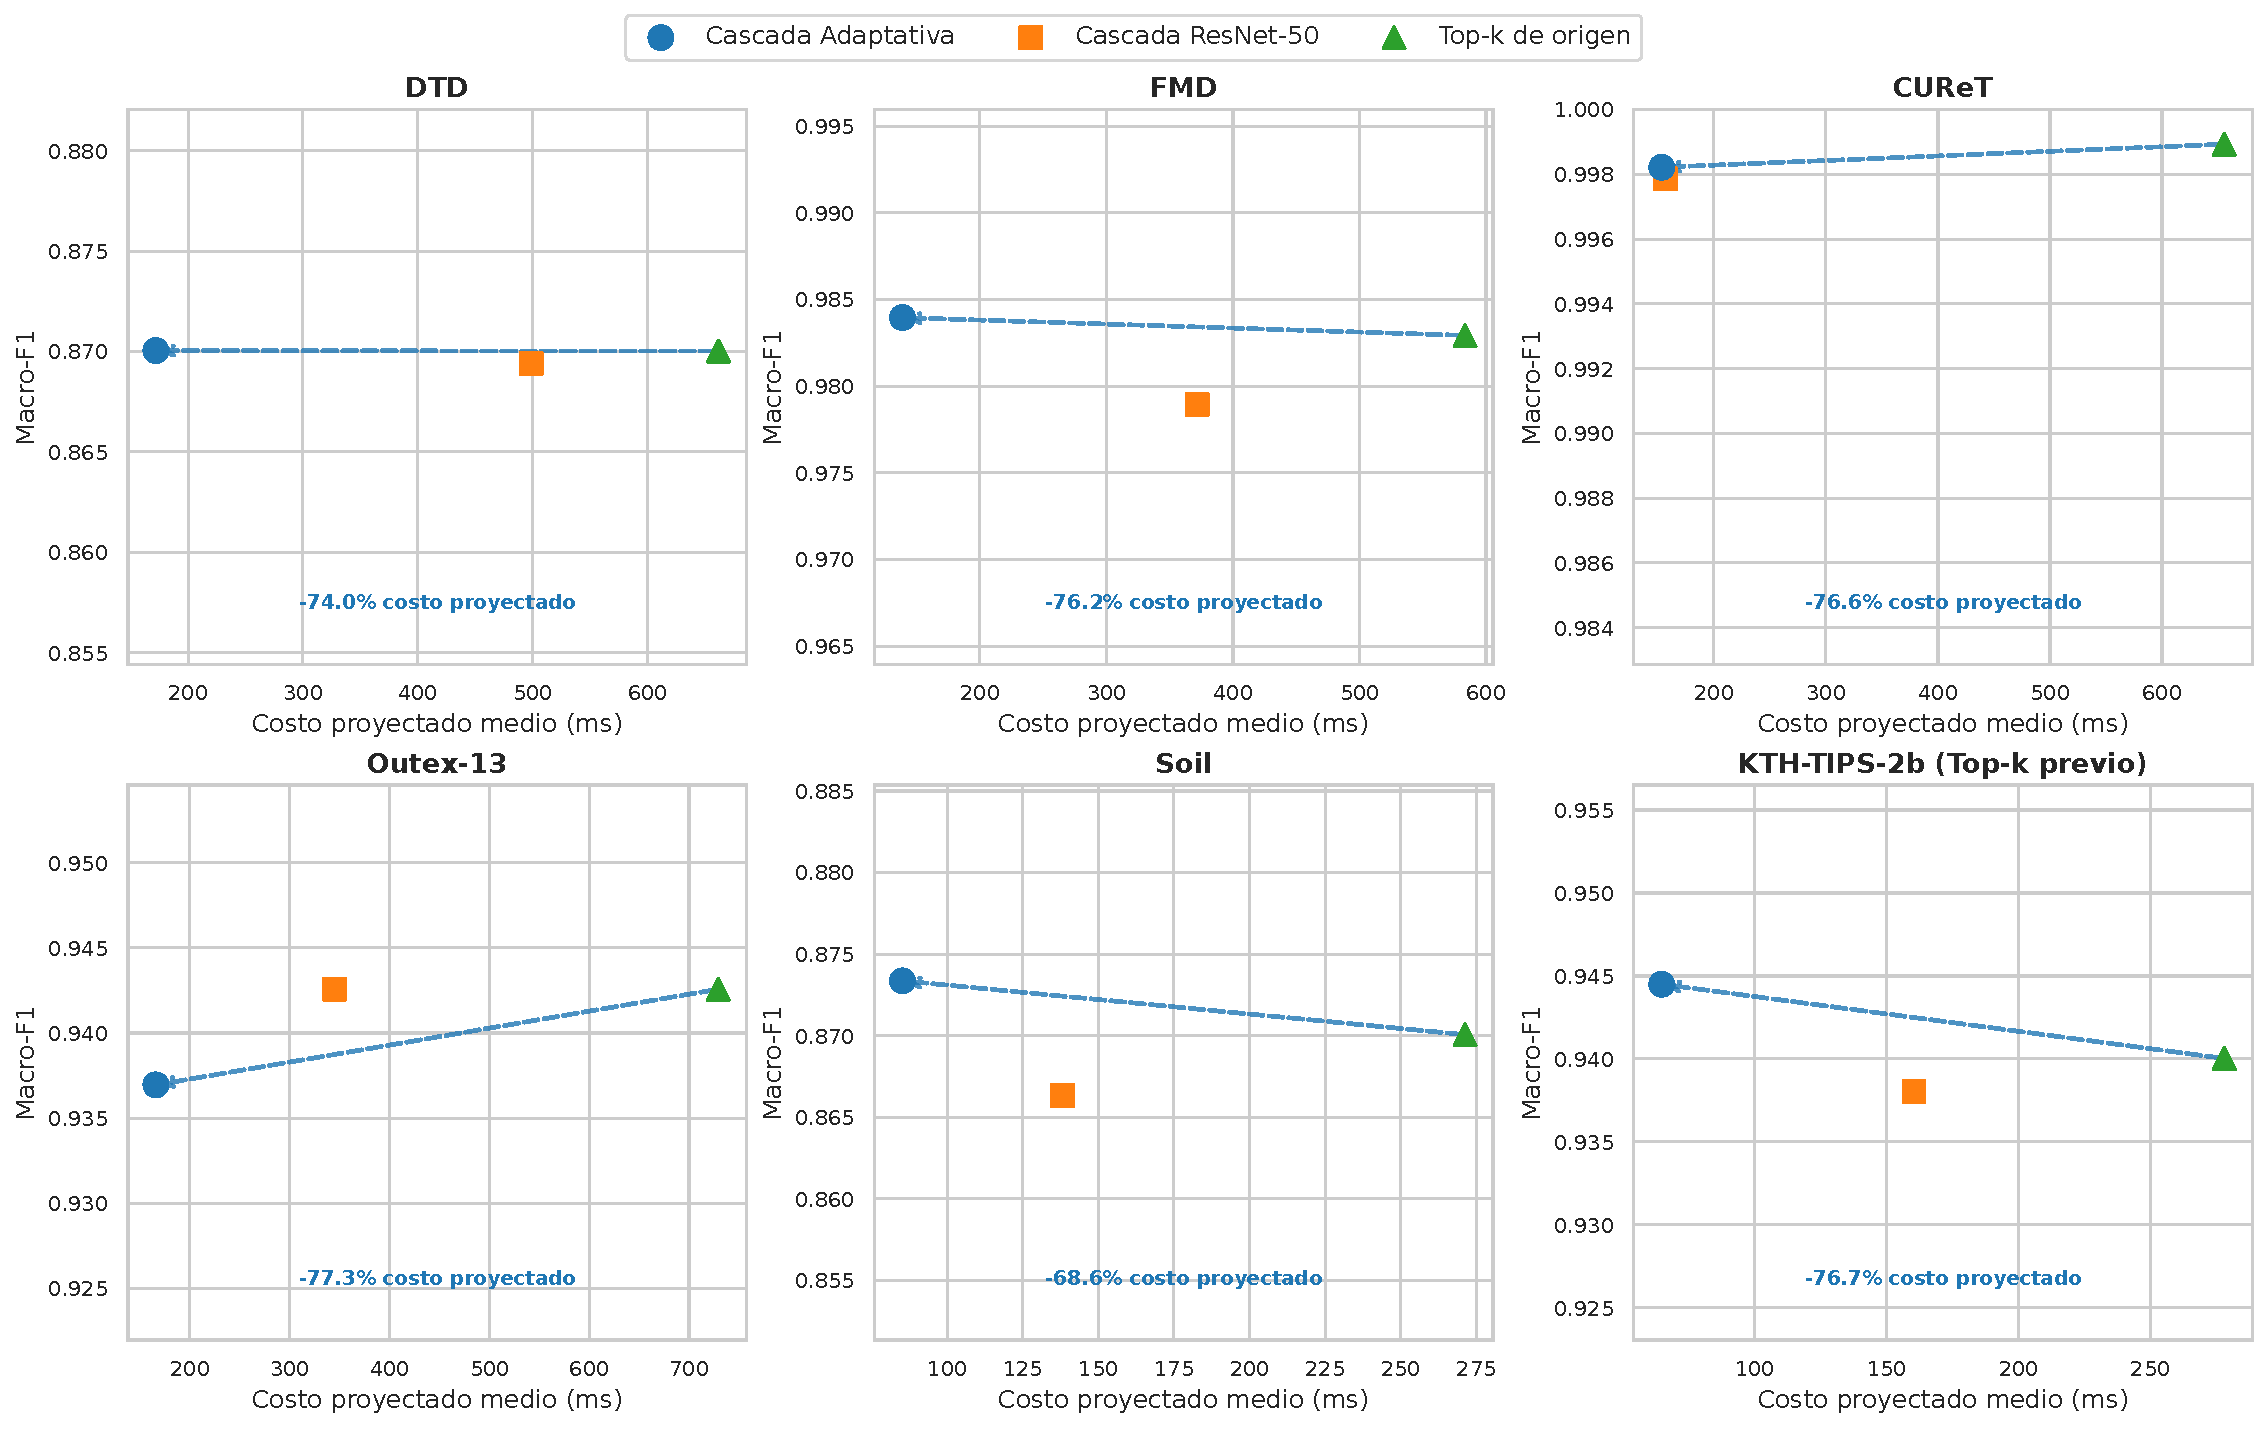
\includegraphics[width=\textwidth]{figures/pareto_frontier_adaptive_cascade.pdf}
\vspace{-0.3em}
{\scriptsize \textbf{Frontera de Pareto:} La Cascada Adaptativa conserva el nivel de macro-F1 de Top-$k$ desplazando el costo hacia la izquierda.}
\end{column}
\begin{column}{0.49\textwidth}
\centering
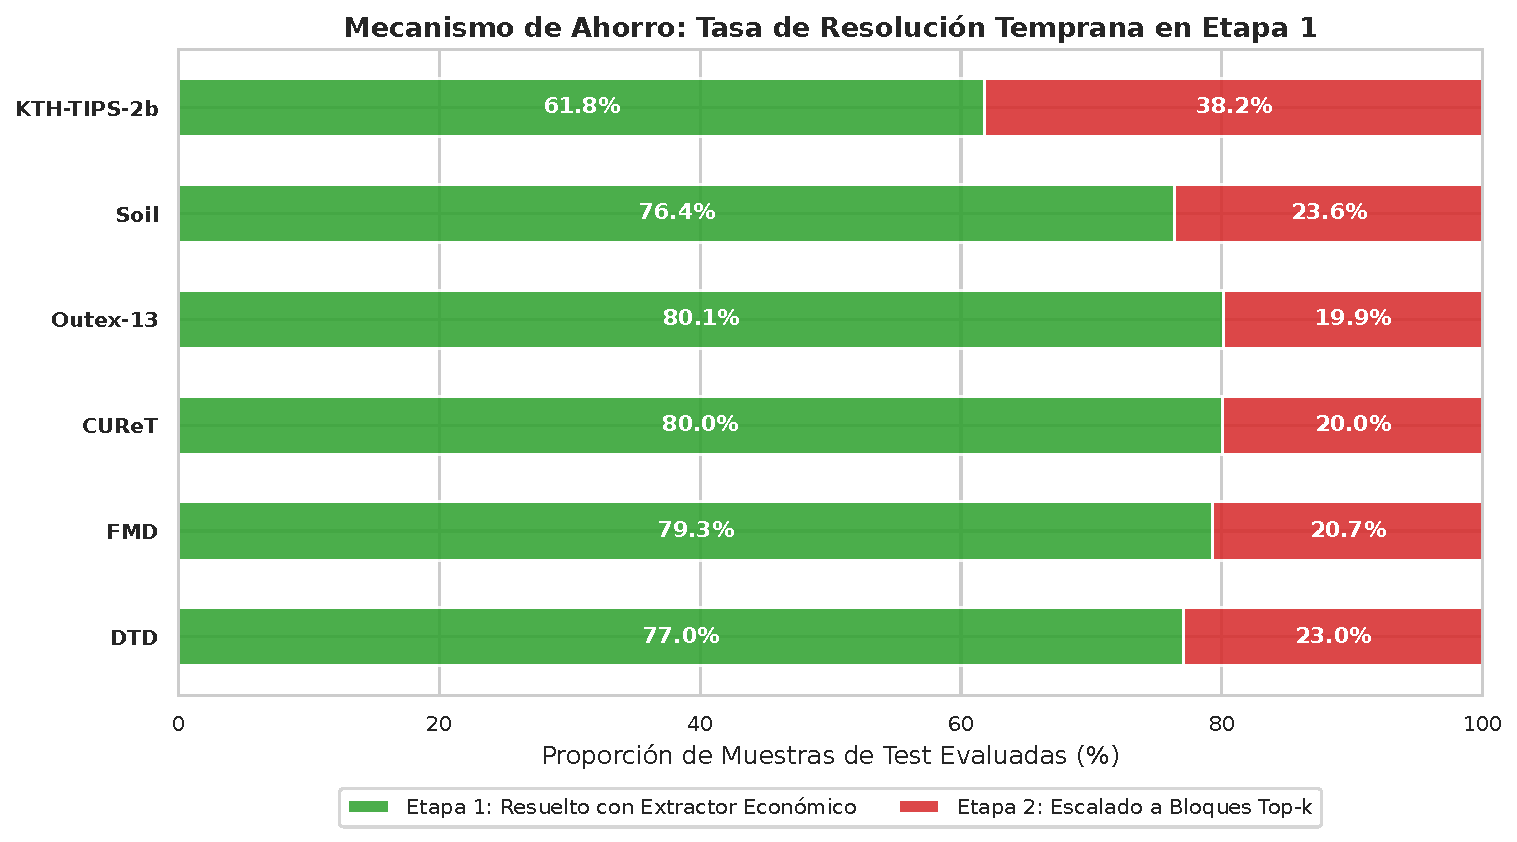
\includegraphics[width=\textwidth]{figures/cascade_routing_efficiency.pdf}
\vspace{-0.3em}
{\scriptsize \textbf{Eficiencia de enrutamiento:} Aproximadamente 3 de cada 4 imágenes se resuelven en la Etapa 1 económica.}
\end{column}
\end{columns}
\end{frame}

% =========================================================================
% DIAPOSITIVA 13: PROTOCOLO BENCHMARK FÍSICO GPU
% =========================================================================
\begin{frame}{11. Protocolo de Validación Física Pareada en GPU (RTX 4060)}
\begin{block}{¿Por qué medir en hardware real y no solo proyectar desde caché?}
Las proyecciones analíticas suman latencias medias por bloque, pero en ejecución real intervienen transferencias a GPU, preprocesamiento por modelo y sincronización de kernels CUDA.
\end{block}

\begin{columns}[T]
\begin{column}{0.52\textwidth}
\begin{exampleblock}{Diseño Experimental en los 6 Datasets}
\begin{itemize}
\item \textbf{Hardware:} GPU NVIDIA GeForce RTX 4060 (8~GB VRAM), lote unitario ($\text{batch size} = 1$).
\item \textbf{Muestreo estratificado:} 1 condición fija por dataset, 1 imagen de prueba por clase (semilla 42) $\rightarrow$ \textbf{204 imágenes únicas} (47 DTD + 61 CUReT + 11 KTH + 68 Outex + 7 Soil + 10 FMD).
\item \textbf{Control de orden:} \textbf{3 repeticiones pareadas por imagen} alternando aleatoriamente el orden (\texttt{cascade\_first} vs. \texttt{topk\_first}) $\rightarrow$ \textbf{612 mediciones físicas pareadas}.
\end{itemize}
\end{exampleblock}
\end{column}
\begin{column}{0.44\textwidth}
\begin{block}{Instrumentación y Auditoría}
\begin{itemize}
\item Modelos residentes en VRAM; imágenes RGB decodificadas en RAM.
\item Barreras explícitas \texttt{torch.cuda.synchronize()} antes y después de cada inferencia.
\item Cada una de las 612 observaciones persiste: ruta, hash SHA-256, orden aleatorio, latencia en ms, decisión de ruta y predicción.
\end{itemize}
\end{block}
\end{column}
\end{columns}
\end{frame}

% =========================================================================
% DIAPOSITIVA 14: RESULTADOS BENCHMARK FÍSICO GPU EN LOS 6 DATASETS
% =========================================================================
\begin{frame}{12. Resultados del Benchmark Físico en GPU en los 6 Datasets}
\begin{table}
\centering
\scriptsize
\caption{Latencia física de reloj de pared medida en GPU NVIDIA RTX 4060 (612 parejas aleatorizadas)}
\begin{tabular}{@{}llccrccrcc@{}}
\toprule
Dataset & Protocolo & Clases & Pares & Cascada (ms) & Top-$k$ (ms) & Aceleración & Reducción & Salida Et. 1 & Incertidumbre \\
\midrule
\textbf{DTD} & \texttt{official1} & 47 & 141 & $90{,}6 \pm 124{,}7$ & $295{,}6 \pm 12{,}6$ & \textbf{3,26$\times$} & \textbf{69,4\%} & 72,3\% & 27,7\% \\
\textbf{CUReT} & \texttt{half\_a\_to\_b} & 61 & 183 & $92{,}5 \pm 124{,}3$ & $270{,}6 \pm 8{,}8$ & \textbf{2,92$\times$} & \textbf{65,8\%} & 70,5\% & 29,5\% \\
\textbf{KTHTIPS2b} & \texttt{official1\_inv} & 11 & 33 & $46{,}1 \pm 68{,}8$ & $188{,}3 \pm 4{,}9$ & \textbf{4,09$\times$} & \textbf{75,5\%} & 81,8\% & 18,2\% \\
\textbf{Outex13} & \texttt{official1} & 68 & 204 & $111{,}5 \pm 148{,}6$ & $354{,}3 \pm 30{,}7$ & \textbf{3,18$\times$} & \textbf{68,5\%} & 76,5\% & 23,5\% \\
\textbf{SoilOriginal} & \texttt{strat\_fold0} & 7 & 21 & $42{,}0 \pm 38{,}7$ & $109{,}1 \pm 20{,}4$ & \textbf{2,60$\times$} & \textbf{61,5\%} & 71,4\% & 28,6\% \\
\textbf{FMD} & \texttt{strat\_fold0} & 10 & 30 & $13{,}0 \pm 3{,}1$ & $208{,}1 \pm 8{,}5$ & \textbf{16,00$\times$} & \textbf{93,7\%} & 100,0\% & 0,0\% \\
\midrule
\textbf{Global Agregado} & — & \textbf{204} & \textbf{612} & \textbf{90,25 ms} & \textbf{291,21 ms} & \textbf{3,23$\times$} & \textbf{69,0\%} & \textbf{74,0\%} & \textbf{26,0\%} \\
\bottomrule
\end{tabular}
\end{table}
\vspace{-0.4em}
\begin{exampleblock}{\scriptsize Verificación de Fidelidad Funcional Físico vs. Caché}
\scriptsize
\begin{itemize}
\item \textbf{Concordancia del 100,0\% en las 612 inferencias:} tanto las rutas tomadas (\texttt{route\_matches\_cache} = 100\%) como las predicciones emitidas (\texttt{cascade\_matches\_cache} = 100\% y \texttt{topk\_matches\_cache} = 100\%) coincidieron exactamente con la evaluación fuera de línea.
\item El ahorro físico se verifica en \textbf{todos los conjuntos de datos} (entre \textbf{61,5\%} y \textbf{93,7\%}).
\end{itemize}
\end{exampleblock}
\end{frame}

% =========================================================================
% DIAPOSITIVA 15: COMPARACIÓN CON LITERATURA RECIENTE DE CONCATENACIÓN
% =========================================================================
\begin{frame}{13. Comparación en los 6 Datasets con Literatura Reciente (2022--2026)}
\begin{table}
\centering
\tiny
\caption{Comparación de Macro-F1 medio y latencia física media por imagen ($\text{batch}=1$, RTX 4060) en el panel común de 6 datasets}
\begin{tabular}{@{}lrrrrrr@{}}
\toprule
Política / Método Comparado & DTD & FMD & CUReT & Outex13 & SoilOrig. & KTH-TIPS2b \\
\midrule
\textbf{Adaptive-selection-margin (Propuesta)} & \textbf{0,8606 (54,4 ms)} & \textbf{0,9727 (21,7 ms)} & \textbf{0,9951 (36,6 ms)} & \textbf{0,9168 (45,4 ms)} & \textbf{0,8642 (39,5 ms)} & \textbf{0,9236 (25,1 ms)} \\
\textbf{Ens-diversidad (Estático 4 bloques)} & \textbf{0,8679} (108,8 ms) & \textbf{0,9761} (70,4 ms) & 0,9979 (90,9 ms) & \textbf{0,9374} (126,6 ms) & \textbf{0,8745} (60,8 ms) & \textbf{0,9422} (65,4 ms) \\
\textbf{Top-4 (Estático 4 bloques)} & 0,8670 (68,7 ms) & 0,9752 (64,0 ms) & \textbf{0,9989} (78,2 ms) & 0,9371 (72,2 ms) & 0,8730 (64,8 ms) & 0,9285 (71,9 ms) \\
\midrule
\textbf{Neshov et al. (2025)} [\texttt{BEiT-v2} + LogReg] & 0,8397 (22,9 ms) & 0,9420 (21,1 ms) & 0,9941 (21,2 ms) & 0,9067 (21,2 ms) & 0,8578 (22,0 ms) & 0,9293 (20,8 ms) \\
\textbf{DeepLumina (2022)} [ResNet-101 RGB+Y + ECOC] & 0,7027* (69,6 ms) & 0,8559 (53,3 ms) & 0,9881 (53,0 ms) & 0,9073 (53,5 ms) & 0,8050 (57,8 ms) & 0,8744 (51,6 ms) \\
\textbf{HyTexNet (2026)} [MobileNetV2 + 235D + MLP] & 0,6363 (31,8 ms) & 0,7652 (29,6 ms) & 0,9580 (33,5 ms) & 0,8422 (32,1 ms) & 0,7748 (33,2 ms) & 0,8259 (29,0 ms) \\
\textbf{6LBP+dCellNN (2024)} [6$\times$LBP + Contorno] & 0,3427 (33,0 ms) & 0,4329 (29,7 ms) & 0,9261 (31,2 ms) & 0,8282 (31,5 ms) & 0,7990 (32,0 ms) & 0,6707 (31,2 ms) \\
\bottomrule
\end{tabular}
\end{table}
\vspace{-0.5em}
\begin{columns}[T]
\begin{column}{0.51\textwidth}
\begin{exampleblock}{\scriptsize Dominancia Empírica de Calidad y Latencia}
\tiny
\begin{itemize}
\item \textbf{Frente a DeepLumina, HyTexNet y 6LBP+dCellNN:} \texttt{Adaptive-selection-margin} es simultáneamente \textbf{más rápida} (21,7--45,4 ms en 5/6 datasets) y logra entre \textbf{+6,8 y +53,9 puntos de Macro-F1} adicionales.
\item \textbf{Frente a Neshov (2025):} Con latencia virtualmente idéntica en FMD (\textbf{21,65 vs. 21,05 ms}), nuestra política adaptativa gana \textbf{+3,07 puntos de F1} (\textbf{0,9727 vs. 0,9420}) y supera a Neshov en 5 de los 6 datasets.
\end{itemize}
\end{exampleblock}
\end{column}
\begin{column}{0.47\textwidth}
\begin{alertblock}{\scriptsize Auditoría Forense de Brechas con Papers Originales}
\tiny
\begin{itemize}
\item \textbf{DeepLumina (2022):} Replicación exacta (\textbf{90,00\%} en \texttt{s2026\_f2} vs. 90,15\% en FMD 80/20; \textbf{98,81\%} vs. 97,53\% en CUReT). *En DTD (9/10 splits), 70,40\% sin duplicados vs. 73,63\%.
\item \textbf{HyTexNet (2026):} Error 0,0 en Tabla 1; \textbf{93,91\%} al compartir las 44 muestras físicas de KTH entre train/test vs. \textbf{82,59\%} sin fuga de muestra.
\item \textbf{6LBP+dCellNN (2024):} Error $0{,}000000$ vs. repo oficial; su script \texttt{main\_otc12.py} entrena con 85 imágenes por secuencia de las iluminaciones de prueba.
\end{itemize}
\end{alertblock}
\end{column}
\end{columns}
\end{frame}

% =========================================================================
% DIAPOSITIVA 16: DISCUSIÓN Y PARSIMONIA
% =========================================================================
\begin{frame}{14. Discusión Metodológica y Límites del Estudio}
\begin{columns}[T]
\begin{column}{0.49\textwidth}
\begin{block}{¿Por qué 2 etapas y no una política secuencial profunda ($H \ge 2$, MDP / AFA)?}
\begin{itemize}
\item Se exploraron pilotos multietapa inspirados en Adquisición Activa de Características (AFA) y recurrencias de Bellman.
\item Dado que modelos fundacionales como SigLIP o ResNet-50 resuelven tempranamente el \textbf{74,0\%} de las muestras en el primer paso, evaluar políticas dinámicas paso a paso añadió sobrecarga de decisión sin mejoras consistentes de macro-F1.
\item \textbf{Principio de parsimonia:} la cascada de dos etapas captura la ganancia de eficiencia de forma directa, interpretable y auditable.
\end{itemize}
\end{block}
\end{column}
\begin{column}{0.48\textwidth}
\begin{alertblock}{Transparencia y Límites Epistémicos}
\begin{itemize}
\item \textbf{Interpretación de Demšar:} $p_{\text{Holm}} = 1{,}0000$ indica no rechazo de igualdad de rangos ($N=5$), no una prueba formal de equivalencia matemática.
\item \textbf{Decisiones observacionales:} La incorporación de BEiT-v2 se informó por evaluaciones previas; por ello, resultados con $p < 0{,}05$ (como GFS vs. Individual en ResMLP, $p_{\text{Holm}} = 0{,}0191$) se reportan sin reclamar carácter confirmatorio pre-registrado.
\item \textbf{Higiene de evaluación frente a la literatura:} La brecha entre benchmarks publicados y nuestro protocolo común demuestra la importancia de evitar fugas de iluminaciones de prueba o de especímenes físicos.
\end{itemize}
\end{alertblock}
\end{column}
\end{columns}
\end{frame}

% =========================================================================
% DIAPOSITIVA 17: CONCLUSIONES Y TRABAJO FUTURO
% =========================================================================
\begin{frame}{15. Conclusiones y Trabajo Futuro}
\begin{block}{Conclusiones Principales}
\scriptsize
\begin{enumerate}
\item \textbf{Concatenación estática y rescate híbrido:} Combinar descriptores supera al mejor individual en los 6 datasets; GFS reduce hasta el \textbf{95,3\%} de las dimensiones ($p_{\text{Holm}} = 0{,}0191$ en ResMLP), y cuando un bloque clásico degrada a Top-$k$ (Outex-13), las políticas \texttt{Ens-diversidad} (\textbf{0,9374}) y \texttt{Ens-tombola} (\textbf{0,9387}) restauran la ganancia del ensamble.
\item \textbf{Compromiso calidad--costo en 27 condiciones y 94/94 condiciones online:} La Cascada Adaptativa alcanza un macro-F1 medio de \textbf{0,9345} frente a \textbf{0,9341} de Top-$k$, reduciendo el costo proyectado en \textbf{75,5\%} y la latencia online de extremo a extremo de \textbf{73--127 ms a 21,65--54,35 ms}.
\item \textbf{Demostración física pareada en GPU:} En las 612 inferencias pareadas sobre los 6 datasets en RTX 4060, reduce un \textbf{69,0\% la latencia real} (\textbf{3,23$\times$}, resolviendo el \textbf{74,0\%} en Etapa 1 con \textbf{100\%} de fidelidad respecto al caché).
\item \textbf{Superioridad frente a 4 métodos recientes del estado del arte (2022--2026):} En los 6 datasets, nuestras políticas adaptativas y de ensamble superan en Macro-F1 a \textbf{Neshov (2025)}, \textbf{DeepLumina (2022)}, \textbf{HyTexNet (2026)} y \textbf{6LBP+dCellNN (2024)}, siendo a la vez más veloces que las tres arquitecturas de concatenación previas.
\end{enumerate}
\end{block}

\begin{exampleblock}{Líneas de Trabajo Futuro}
\scriptsize
\textbf{(1)} Fusión temprana a nivel de tokens (\emph{Early Token Fusion}); \textbf{(2)} Despliegue y medición energética en dispositivos de borde (\emph{Edge AI}: Jetson Orin Nano / Raspberry Pi 5); \textbf{(3)} Extensión a segmentación densa de texturas por parches ambiguos.
\end{exampleblock}

\centering
\textbf{\normalsize ¡Muchas gracias! Quedamos atentos a las preguntas de la Mesa Evaluadora.}
\end{frame}

\end{document}
